\chapter{Környezet}

Ebben a fejezetben bemutatom azokat a technológiákat, melyek szükségesek a programom technikai oldalának megértéséhez. Először ismertetem a Control Flow Automata ábrázolás részleteit (Alfejezet \ref{sec:kornyezet_cfa}), aztán kitérek a Theta keretrendszerre (Alfejezet \ref{sec:kornyezet_theta}).

\section{Control Flow Automata}
\label{sec:kornyezet_cfa}

A programkódokat sokféleképpen ábrázolhatjuk \cite{soft_ver_akos}. Legismertebb a programkód, melyet az ember könnyen, gyorsan tud olvasni illetve írni, ellenben a bájtkóddal, melyet a számítógép tud jóval hatékonyabban kezelni. Szoftververifikáció terén is létezik...

\subsection{Példák CFA alkalmazásra}
\label{sec:kornyezet_peldak}

\begin{itemize}
	\item Szoftver
	
	\item Hardver
	
	\item Protokoll
\end{itemize}

\section{Theta keretrendszer}
\label{sec:kornyezet_theta}

A \emph{Theta}\footnote{\url{https://github.com/FTSRG/theta}} egy nyílt forráskódú, általános célú, moduláris és konfigurálható modellellenőrző keretrendszer, melyet absztrakciós finomításon alapuló algoritmusok tervezésének és értékelésének támogatására hoztak létre a különböző formalizmusok elérhetőségi elemzéséhez.

A keretrendszer a már évek óta tartó fejlesztéseknek köszönhetően számos eszközt tud nyújtani modellellenőrzéshez:\footnote{2020 decemberének elején.}

\begin{itemize}
	\item \verb+theta-cfa-cli+ -- Control Flow Automata hibahelyeinek\footnote{Az angol irodalom a \emph{location} kifejezést használja. Én a dolgozatomban a magyar megfelelőjét használom.} elérhetőségét vizsgálja CEGAR alapú algoritmusokkal
	
	\item \verb+theta-sts-cli+ -- \emph{Symbolic Transition Systems} biztonsági tulajdonságainak verifikációját végzi CEGAR alapú algoritmusokkal
	
	\item \verb+theta-xta-cli+ -- Uppaal időzített automaták verifikációját lehet vele elvégezni
	
	\item \verb+theta-xsts-cli+ -- \emph{eXtended Symbolic Transition Systems} biztonsági tulajdonságainak verifikációját végzi CEGAR alapú algoritmusokkal
\end{itemize}
\ \\
A Theta architektúrája négy rétegre osztható. Nevezetesen:

\begin{itemize}
	\item \textbf{Formalizmusok} -- A Theta legalapvetőbb elemei, melyek való-életbeli problémákat modelleznek le, ahogy azt az előző fejezetben láthattuk (Al-alfejezet \ref{sec:kornyezet_peldak}). A formalizmusok általában alacsony szintű, matematikai ábrázolások melyek elsőrendű logikai kifejezéseken és gráfszerű struktúrákon alapulnak. Ilyen például a \emph{Symbolic Transition Systems} 

	\item \textbf{Háttéranalízis} -- 
	
	\item \textbf{SMT megoldó} -- 
	
	\item \textbf{Eszközök} -- Parancssori alkalmazások melyek futtatható \verb+jar+ fájlba fordíthatóak le. Jellemzően csak beolvassák az inputot és meghívják az alsóbb szinten lévő algoritmusokat. 
	
\end{itemize}




























\begin{comment}
\begin{figure}[h]
	\centering
	\begin{lstlisting}[style=CStyle]
		#include <stdio.h>
		int main(void)
		{
			printf("Hello World!"); 
		} \end{lstlisting}
	\caption{My code.}
	\hfill
	\subfloat[Flower two.]{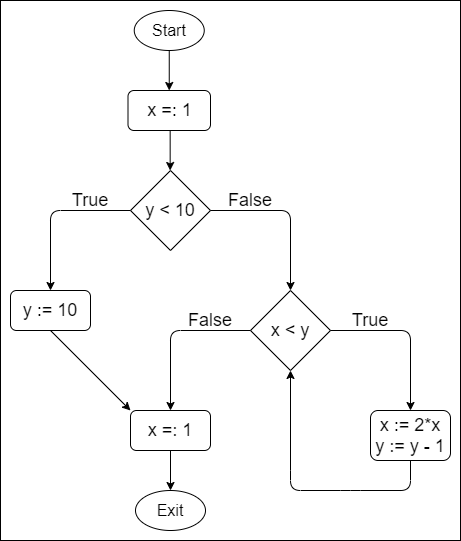
\includegraphics[width=0.4\textwidth]{figures/cfg.png}\label{fig:cfg}}
	\caption{My flowers.}
\end{figure}
\end{comment}